\documentclass{article}

\usepackage[margin=1in]{geometry}
\usepackage[utf8]{inputenc}
\usepackage[english]{babel}
\usepackage{amsthm} %lets us use \begin{proof}
\usepackage{amssymb} %gives us the character \varnothing
\usepackage{xcolor}
\usepackage{float}
\usepackage{braket}
\usepackage{multirow}
\usepackage{array}
\usepackage{mathtools}

\title{Chem231B: Quiz \#4} % Title of the assignment

\begin{document}

\maketitle

\begin{enumerate}
\item What is the spin multiplicity of the ground state of H$_2$ and
  of H$_2^+$?

  {\color{blue} H$_2$ spin multiplicity is 1; H$_2^+$ is 2.}
  
\item Give the electronic Hamiltonian for H$_2$.

  {\color{blue} $H_{\text{el}} = \hat{h}(1) + \hat{h}(2) + V_{ee}$
    where $\hat{h}(i)$ is the one electron Hamiltonian for $i$-th electron
    and $V_{ee}$ is the coulombic interaction:
    
    $\hat{h}(i) = -\frac{\nabla_i^2}{2}-\frac{1}{|r_i - R\hat{z}|} -\frac{1}{|r_i|}$
    and $V_{ee} = \frac{1}{|r_1 - r_2|}$

    $r$ is the position of the electron and $R$ is the position of the
    nucleus. The H$_2$ is placed along the z-axis where a proton is at the origin.
  }
\item Which one of the following changes significantly when going from
  H$_2$ to D$_2$:  $R_e$, $D_e$, $\omega$?

  {\color{blue} $\omega$.}
\item Within the harmonic approximation, say how your answer to the previous
  question will change?

  {\color{blue} Still $\omega$.}
\item Give an expression for the matrix element $H_{AA}$ in H$_2^+$ for
  1s orbitals ($\gamma=1$).

  {\color{blue}
  $h_{AA} = \gamma^2/2 - \gamma f(x) = 1/2 - f(x)$,
  where $f(x) = 1-\frac{(1+x)e^{-2x}-1}{x}$}.
\item Sketch how the matrix element $H_{AA}$ should depend on $R$, giving its
  value as $R\to\infty$.
  \begin{center}
    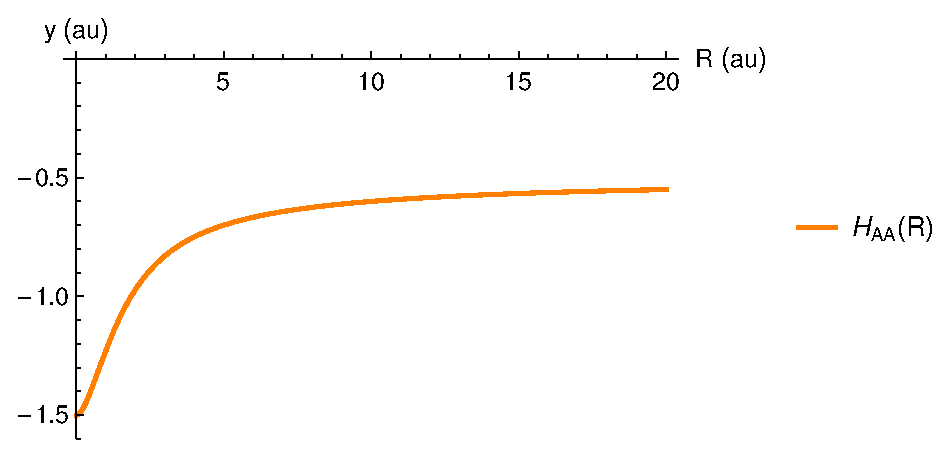
\includegraphics[scale=0.5]{haa_quiz4.eps}
  \end{center}
  {\color{blue}$H_{AA}$ should go to -0.5 Hartree as $R \rightarrow \infty$.}
\item Sketch a molecular energy curve for $H_2$ as a function of $R$,
  giving its value as $R\to\infty$.
  \begin{center}
    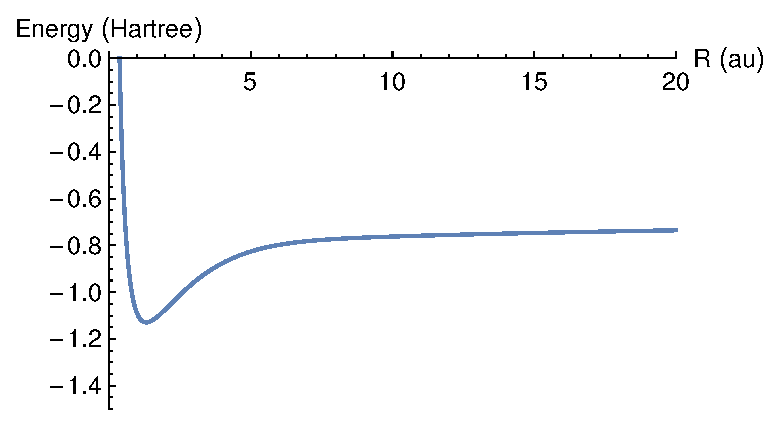
\includegraphics[scale=0.5]{hf_energy.eps}
  \end{center}
  {\color{blue} -11/16 or -0.6875 Hartree as $R\rightarrow \infty$}
\item Sketch the curve within the Hartree-Fock approximation.
  What qualitative error does it make?

  {\color{blue}\textit{Sketch which curve within HF?}}

\item For a molecule with $y_e=0$, deduce a formula for the number of
  states it will bind in terms of $D_e$, $\omega$, and $x_e$.

  {\color{blue}
  $E_{\text{vib}}(\nu) = \nu_e[(\nu +1/2) - x_e(\nu+1/2)^2]$

  Dissociation is when $E_{\text{vib}} = D_e$ and hence, solve for $\nu$ which
  will yield the max number of bounded states
  $\nu_{\text{max}} \approx \frac{1}{2x_e} - \frac{1}{2} + 
  \frac{\sqrt{(1-x_e)^2-4x_eD_e/\nu_e}}{2x_e}$}
  
\item Deduce an expression for $x_e$ in terms of $D_e$ and $\omega$
for the Morse potential, for which 
$
\epsilon_n = -V_0\, \left( 1 - \frac{\alpha (n+\frac{1}{2})}{\sqrt{2\, \mu\, V_0}} \right)^2
$

{\color{blue}
$x_e = \frac{\omega}{8 D_e}$}
\end{enumerate}
  
  
  
\end{document}
